
\section{Хөгжүүлэлт}
\subsection{Хөгжүүлэлтийн орчныг бэлдэх}
Энэхүү судалгааны ажлын практик хэсэгт би NextJS, Hardhat, Pinata IPFS, Lit Protocol, Wagmi, Tailwind CSS зэргийг ашиглан хөгжүүлэлт хийх билээ. NextJS нь монолитик төсөл хийхэд тохиромжтой ба төслийн ухаалаг гэрээн хөгжүүлэлт, клайнт талуудыг нэг repository-д хадгалж байгаа. Version Control System-ээр Github-г сонгосон юм. Кодын фолдер бүтэц нь дараах байдлаар байна.

\begin{figure}[htbp]
   \centering
   \begin{minipage}[ht]{0.4\textwidth}
       \centering
       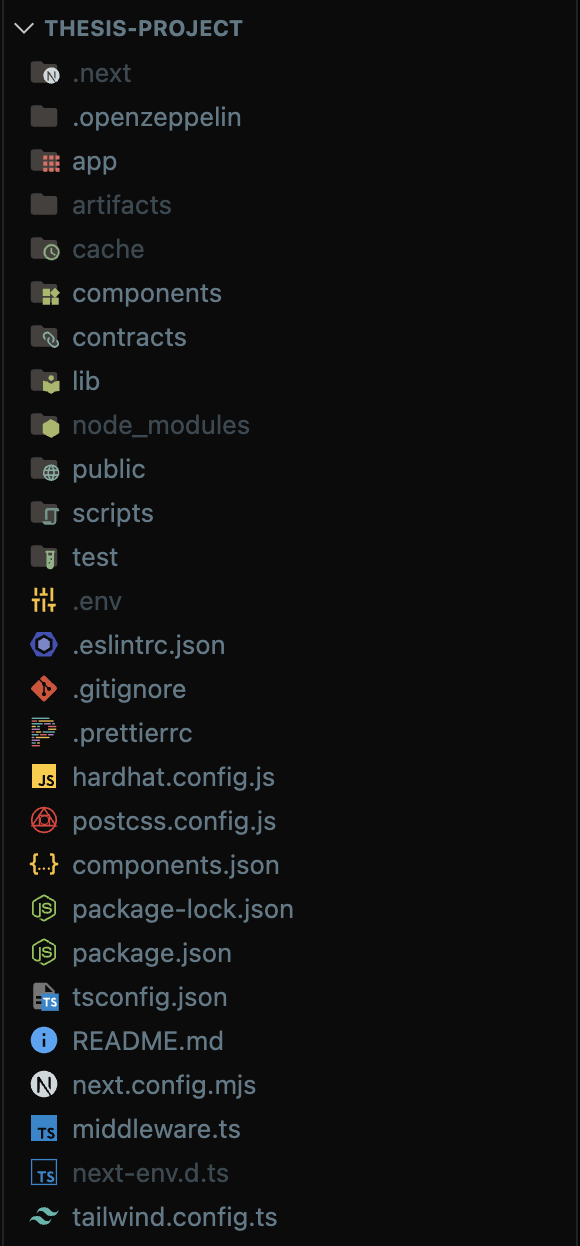
\includegraphics[scale=0.27]{src/images/folder-structure.png}
       \caption{Хөгжүүлэлтийн орчин}
   \end{minipage}
   \begin{minipage}[h!t]{0.5\textwidth}
      \raggedright
      \begin{itemize}
         \item \textbf{components} - React компонентууд
         \item \textbf{lib} - Хэрэглэгчийн талын шаардлагатай код туслах функцүүд
         \item \textbf{app} - NextJS дээрх хуудаснууд
         \item \textbf{public} - Статик зураг, файлууд
         \item \textbf{scripts} - Ухаалаг гэрээний хөгжүүлэлттэй холбоотой  javascript файлууд
         \item \textbf{contracts} - Ухаалаг гэрээний файлууд
      \end{itemize}
  \end{minipage}
\end{figure}

\newpage
\subsection{Ухаалаг гэрээн хөгжүүлэлт}
Миний төсөл нэг ухаалаг гэрээнээс бүтнэ. Ухаалаг гэрээг Solidity хэл дээр бичсэн бөгөөд Ethereum  блокчэйн дээр байршуулсан. Уг ухаалаг гэрээ нь цахим файлууд болон тэдгээртэй холбоотой лицензүүдийг төлөөлдөг Файл ба Лиценз гэсэн хоёр бүтцийг тодорхойлсон. Файл бүтэц  нь id, эзэмшигчийн хаяг, файлын нэр, дэлгэрэнгүй, ангилал, шифрлэсэн файлын хэш, файлын хэмжээ, үүсгэсэн хугацаа зэрэг атрибутуудыг агуулна. Лиценз бүтэц нь лицензийн дугаар, бүтээл эзэмшигчийн хаяг, лиценз эзэмшигчийн хаяг, файлын нэр, дэлгэрэнгүй, ангилал, шифрлэсэн файлын хэш, файлын хэмжээ, үүсгэсэн хугацааны  зэрэг атрибутуудыг агуулна.
Мөн дараах функцүүдтэй:

\begin{table}[h!]
	\centering
   \begin{tabularx}{\textwidth}{|p{0.35\textwidth}|X|}
		\hline
		 \textbf{createFile}& Цахим бүтээлийн мэдээллийг бичих
	\\ \hline \textbf{getAllPublicFiles} & Оруулсан бүх цахим бүтээлийн мэдээллийг авах
	\\ \hline \textbf{getAllUserFiles} &  Хэрэглэгчийн оруулсан цахим бүтээлийн мэдээллийг авах
	\\ \hline \textbf{getAllUserLicenses} & Хэрэглэгчийн эзэмшиж буй цахим бүтээлийн лицензүүдийг авах
	\\ \hline \textbf{getPublicFileById} & Цахим бүтээлийн мэдээллийг дугаараар нь авах
	\\ \hline \textbf{requestLicense} & Цахим бүтээлийг авах бүтээлийн эзэмшигч рүү лицензийн хүсэлт илгээх
	\\ \hline \textbf{approveLicenseRequest} & Өөрийн цахим бүтээлд ирсэн хүсэлтийг зөвшөөрөх
	\\ \hline \textbf{rejectLicenseRequest} & Өөрийн цахим бүтээлд ирсэн хүсэлтээс татгалзах
	\\ \hline \textbf{getFileOwnerLicenseRequests} & Бүтээлийн эзэмшигчид ирсэн хүсэлтүүдийг авах
	\\ \hline \textbf{isFileOwnedOrLicensed} & Цахим бүтээлийн эзэмшигч эсэх эсвэл түүний лицензийг авсан эсэхийг шалгах
	\\ \hline \textbf{generateUniqueLicense} & Лицензэд өвөрмөц дугаар бий болгох                                                             \\ \hline
	\end{tabularx}
   \caption{Ухаалга гэрээний функцүүд}
\end{table}

\newpage
\subsection{Ухаалаг гэрээг этереум блокчэйнд байршуулах}
\lstinputlisting[language=TypeScript,caption=Ухаалаг гэрээг блокчэйнд байршуулах,basicstyle=\linespread{0.6}\ttfamily,frame=single]{src/code/deploy.js}

\subsection{Lit protocol-н файл шифрлэлт болон хандалтын хяналтын нөхцөл}
Lit Protocol-оор дамжуулан клиент талд файлыг шифрлэх ба блокчэйнд байршуулсан ухаалаг гэрээний функцийг ашиглан файлыг зөвхөн бүтээл эзэмшигч эсвэл тухайн бүтээлд лиценз буюу хандах зөвшөөрөлтэй хэрэглэгч эсэхийг баталгаажуулан файлын шифрлэлтийг тайлан харах боломжтойгоор хандалтын хяналтын нөхцөлийг тодорхойлсон.

\lstinputlisting[language=TypeScript,caption=Lit protocol-н файл шифрлэлт болон хандалтын хяналтын нөхцөл,basicstyle=\linespread{0.6}\ttfamily,frame=single]{src/code/lit.ts}


\subsection{Файлыг IPFS-д хадгалах}
\lstinputlisting[language=TypeScript,caption=Файлыг IPFS-д хадгалах,basicstyle=\linespread{0.6}\ttfamily,frame=single]{src/code/uploadIpfs.ts}

\subsection{Ухаалаг гэрээнээс өгөгдлийг унших}
Wagmi-н тодорхойлсон React Hook-г ашиглан цахим бүтээл эзэмшигчийн оруулсан бүтээлүүдийг ухаалаг гэрээнээс уншина.
\lstinputlisting[language=TypeScript,caption=Ухаалаг гэрээний өгөгдлийг унших,basicstyle=\linespread{0.6}\ttfamily,frame=single]{src/code/getUserFiles.ts}


\newpage
\section{Үр дүн}
Хөгжүүлэлтийг дээрх бүлэг сэдвүүд дээр тодорхойлсон шинжилгээ, зохиомжийн дагуу хийсэн болно. Системийн интерфейс дараах байдлаар харагдана.

\begin{figure}[h!]
	\centering
	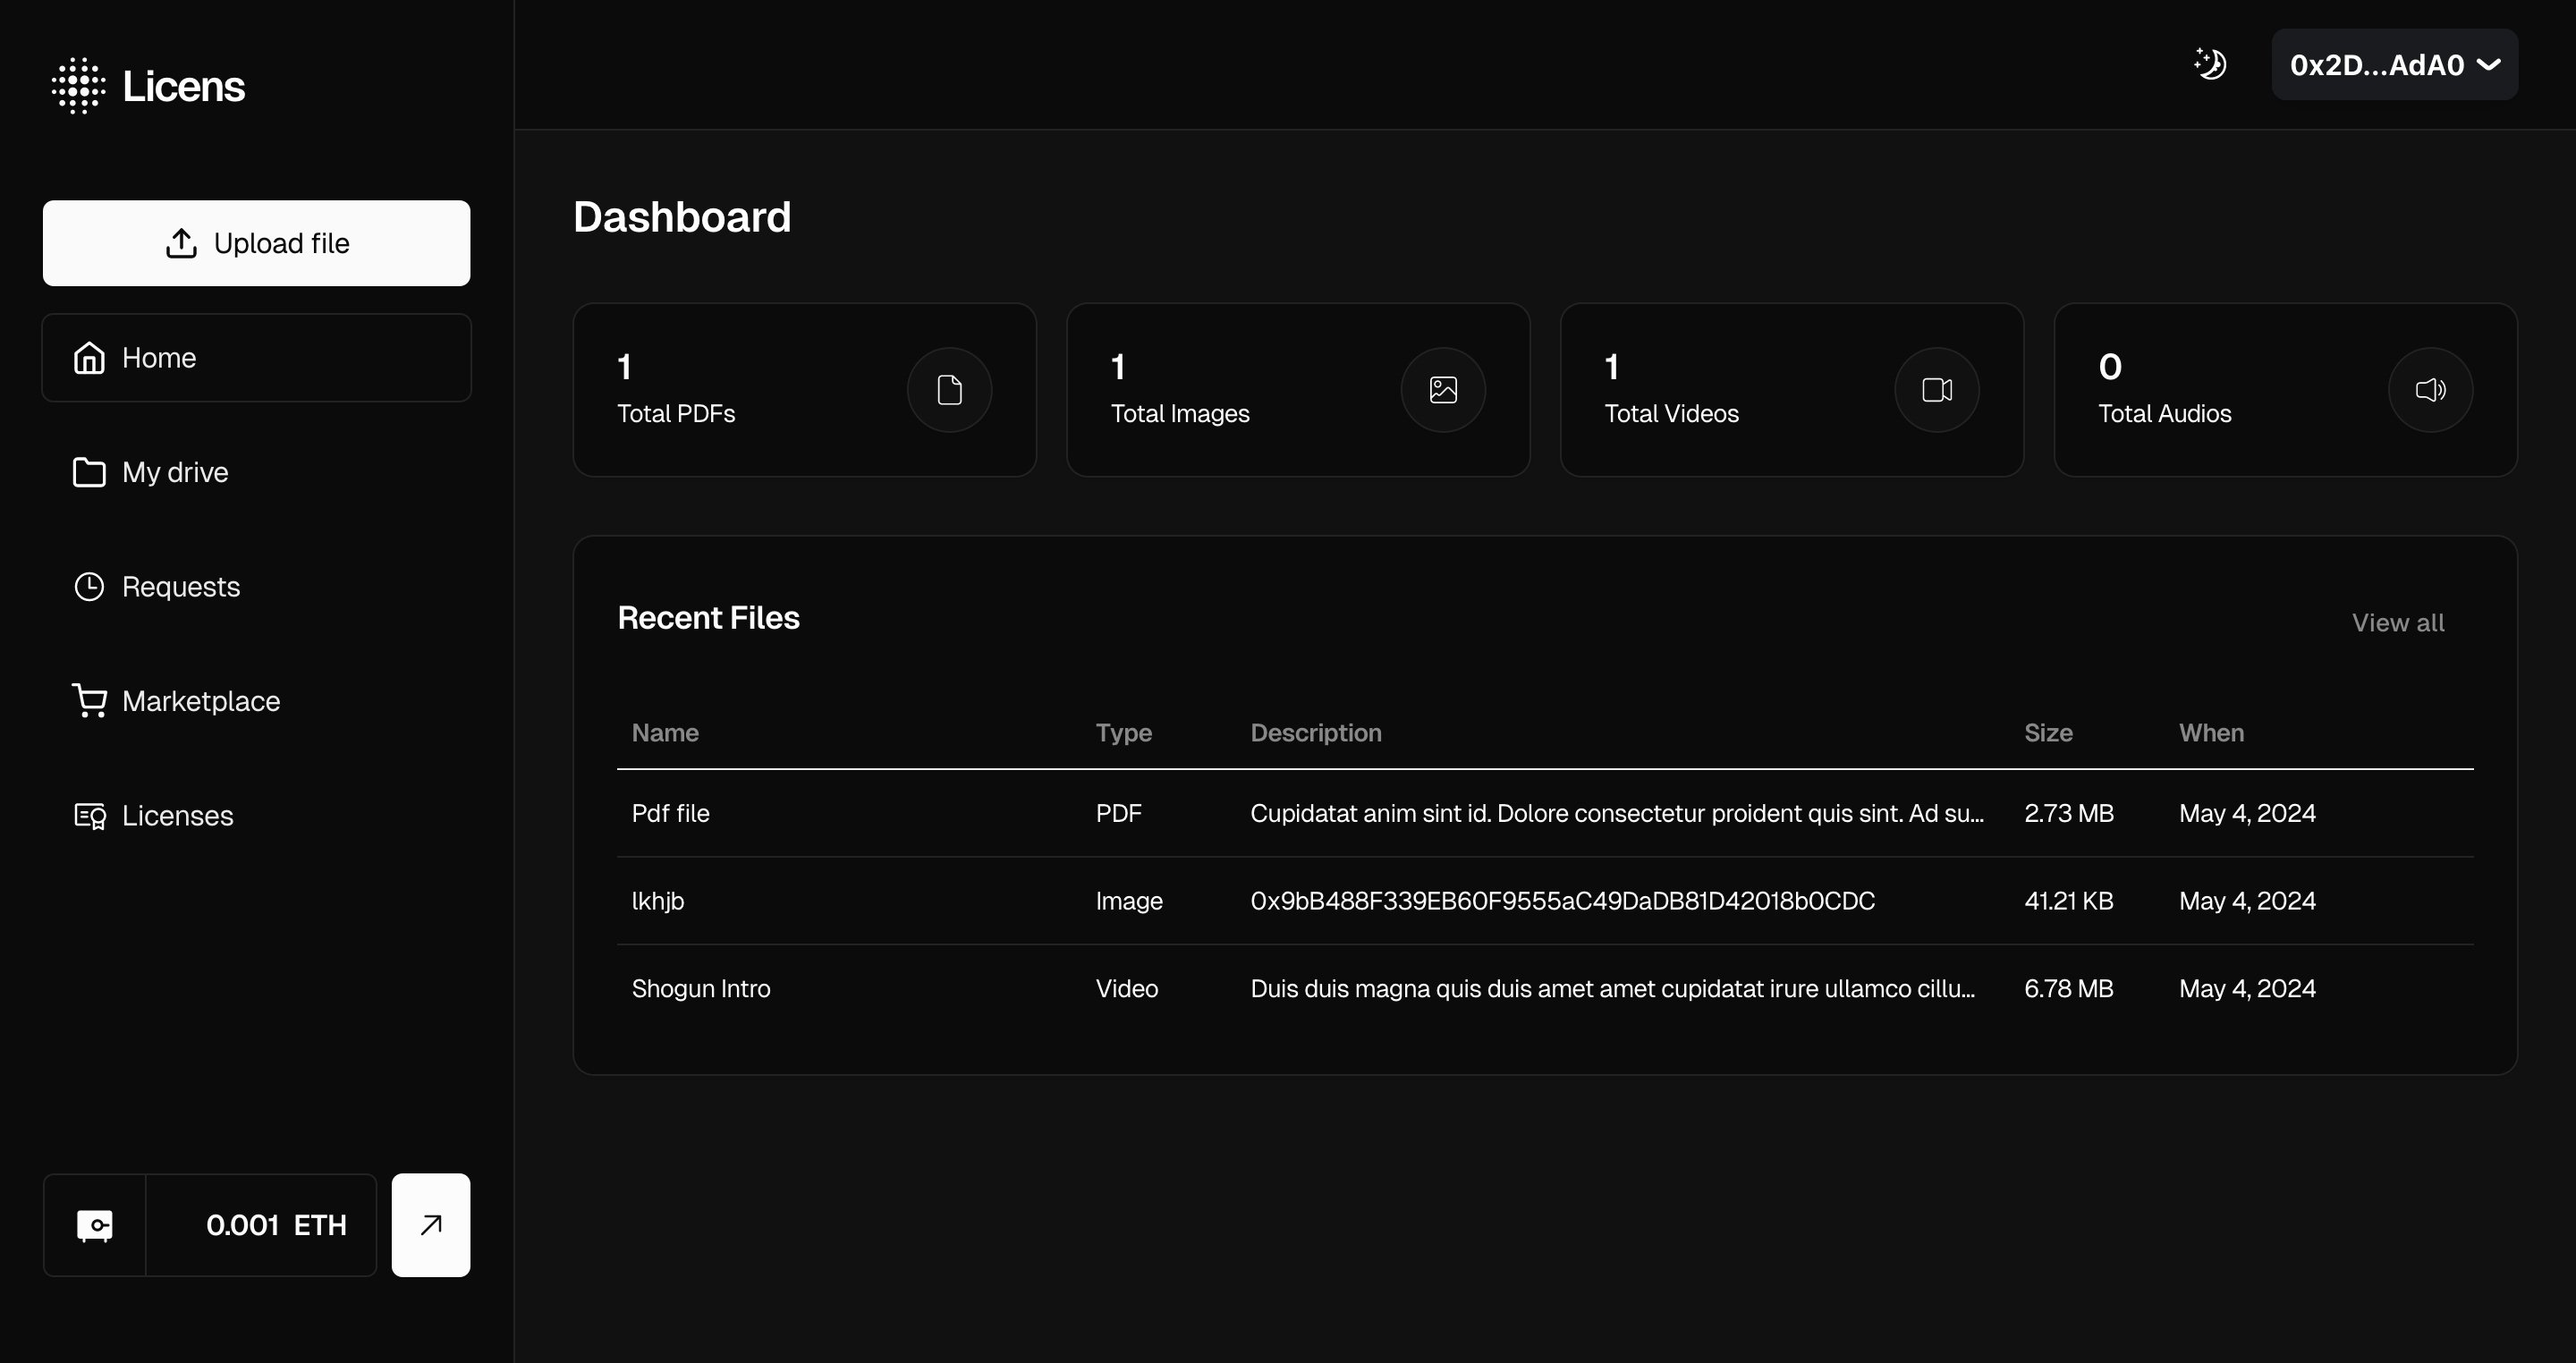
\includegraphics[scale=0.15]{src/images/dashboard.png}
	\caption{Хэрэглэгчийн үндсэн хуудас}
\end{figure}

% \subsubsection{Цахим бүтээл оруулах хуудас}
\begin{figure}[h!]
	\centering
	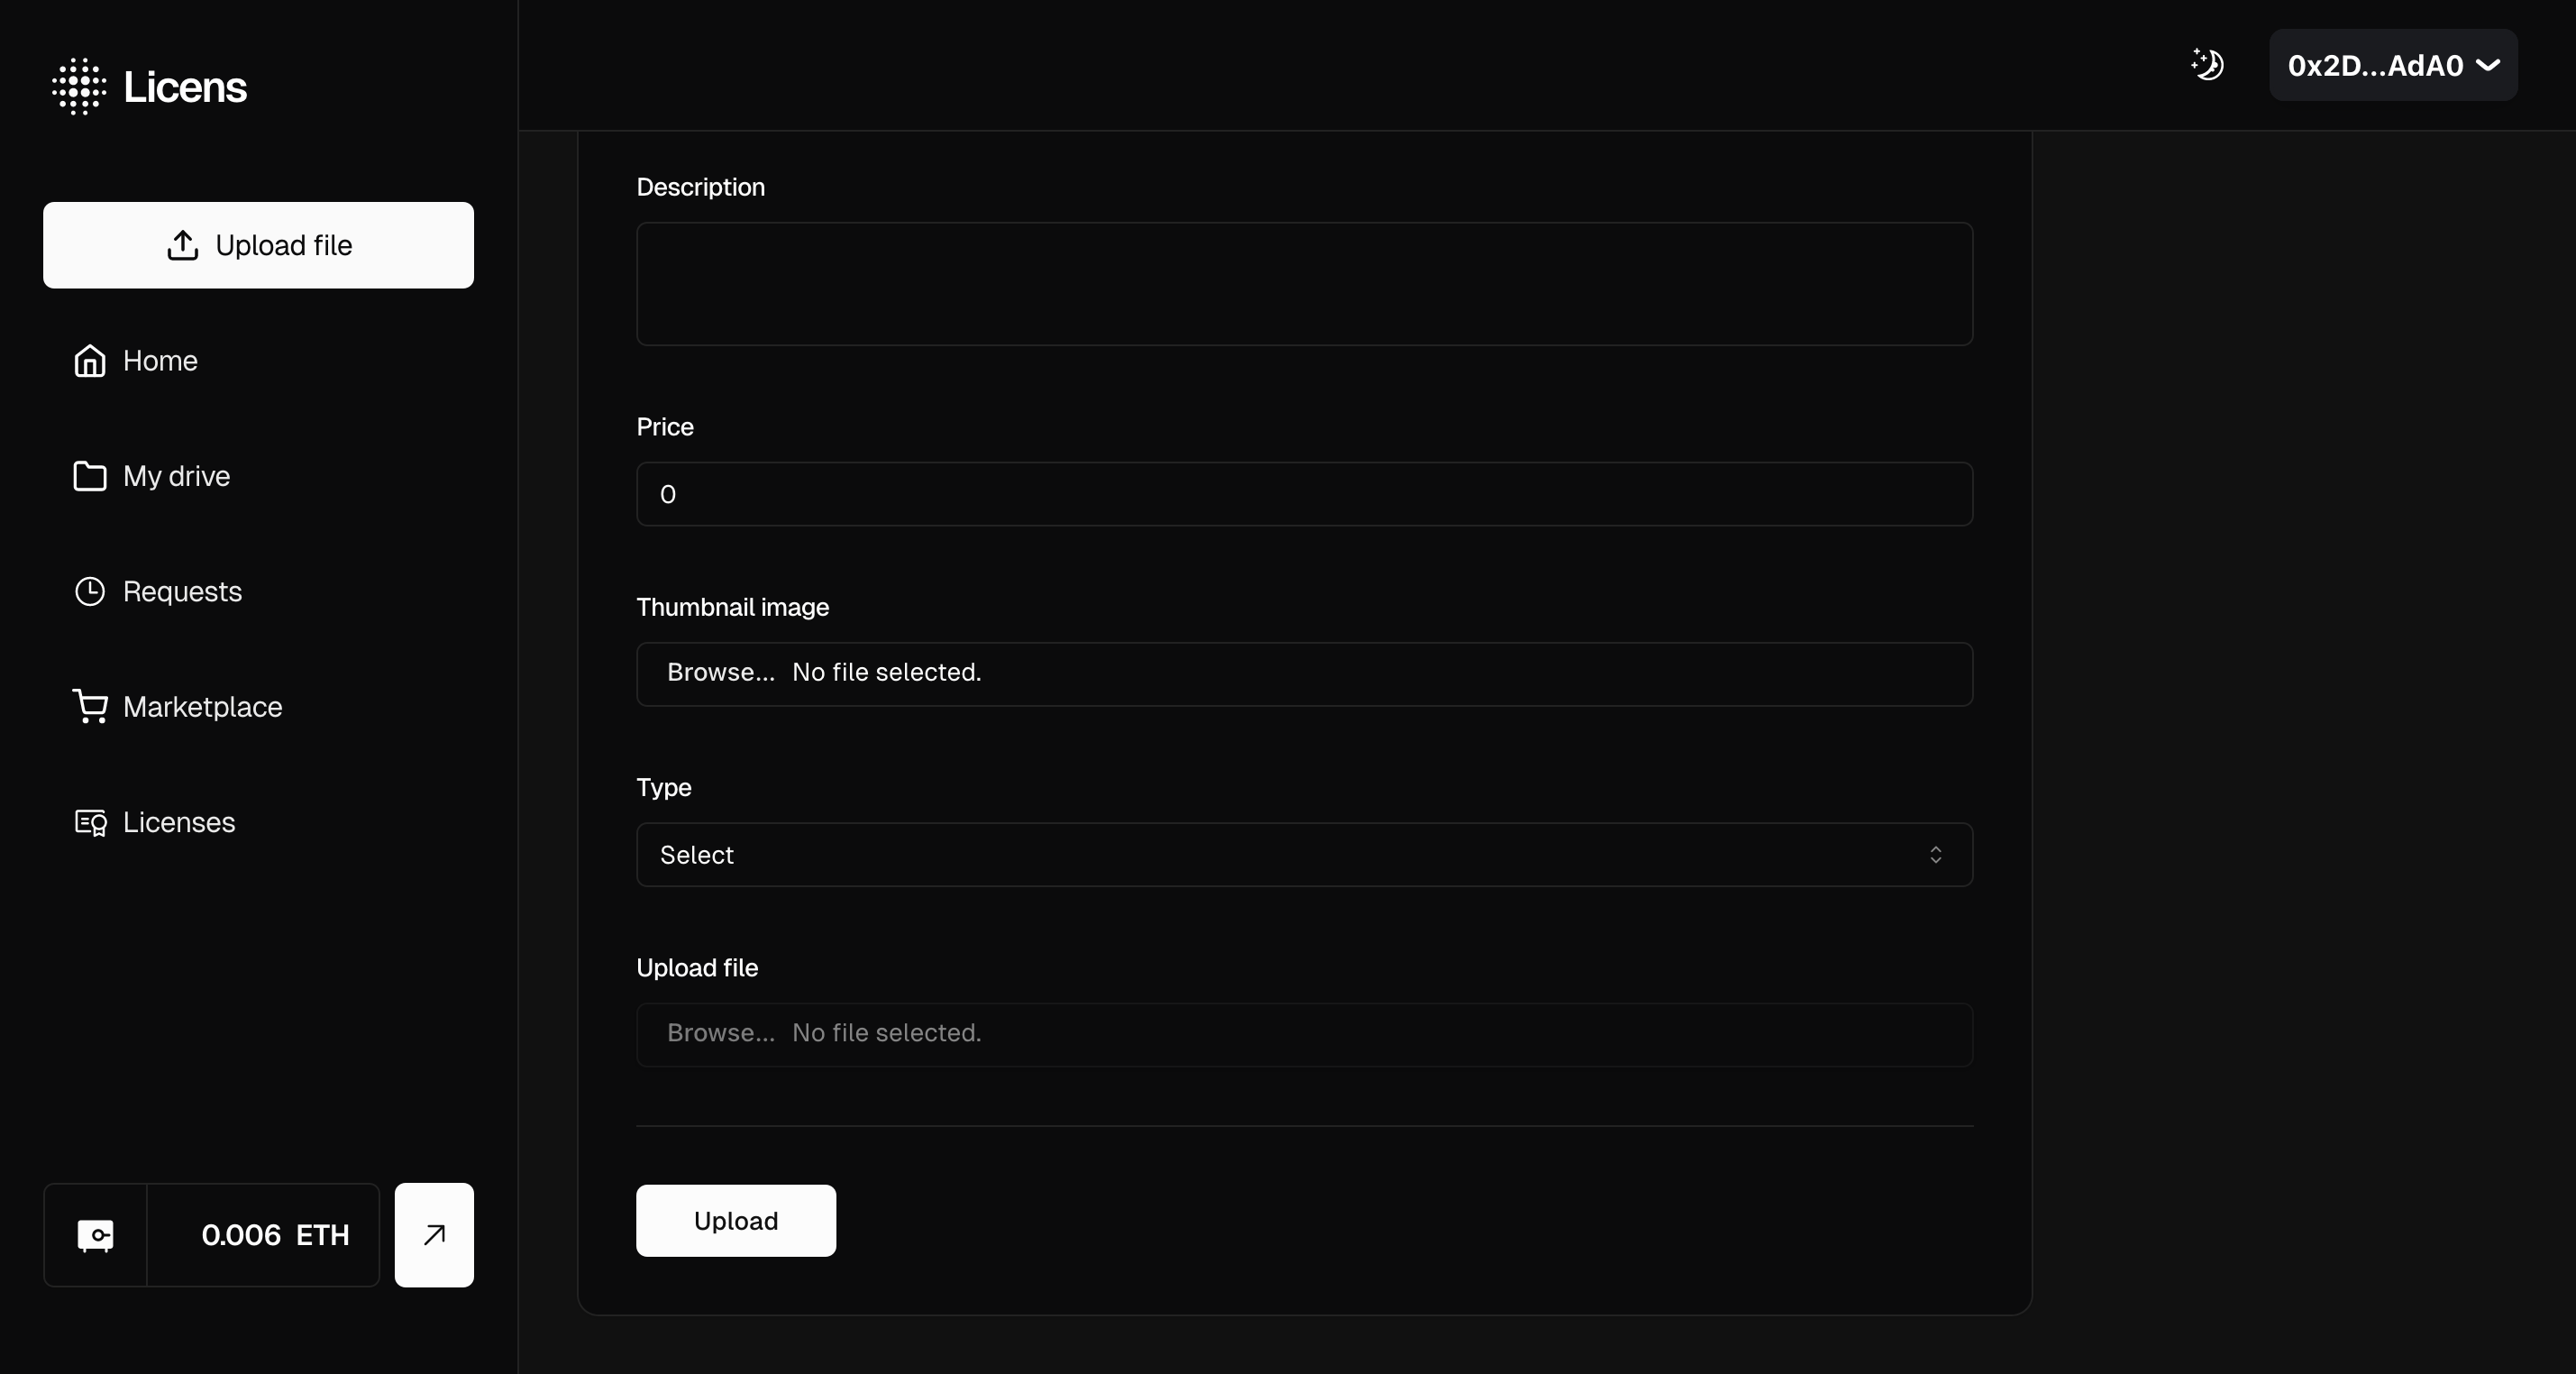
\includegraphics[scale=0.15]{src/images/upload.png}
	\caption{Цахим бүтээл оруулах хуудас}
\end{figure}

\begin{figure}[h!]
	\centering
	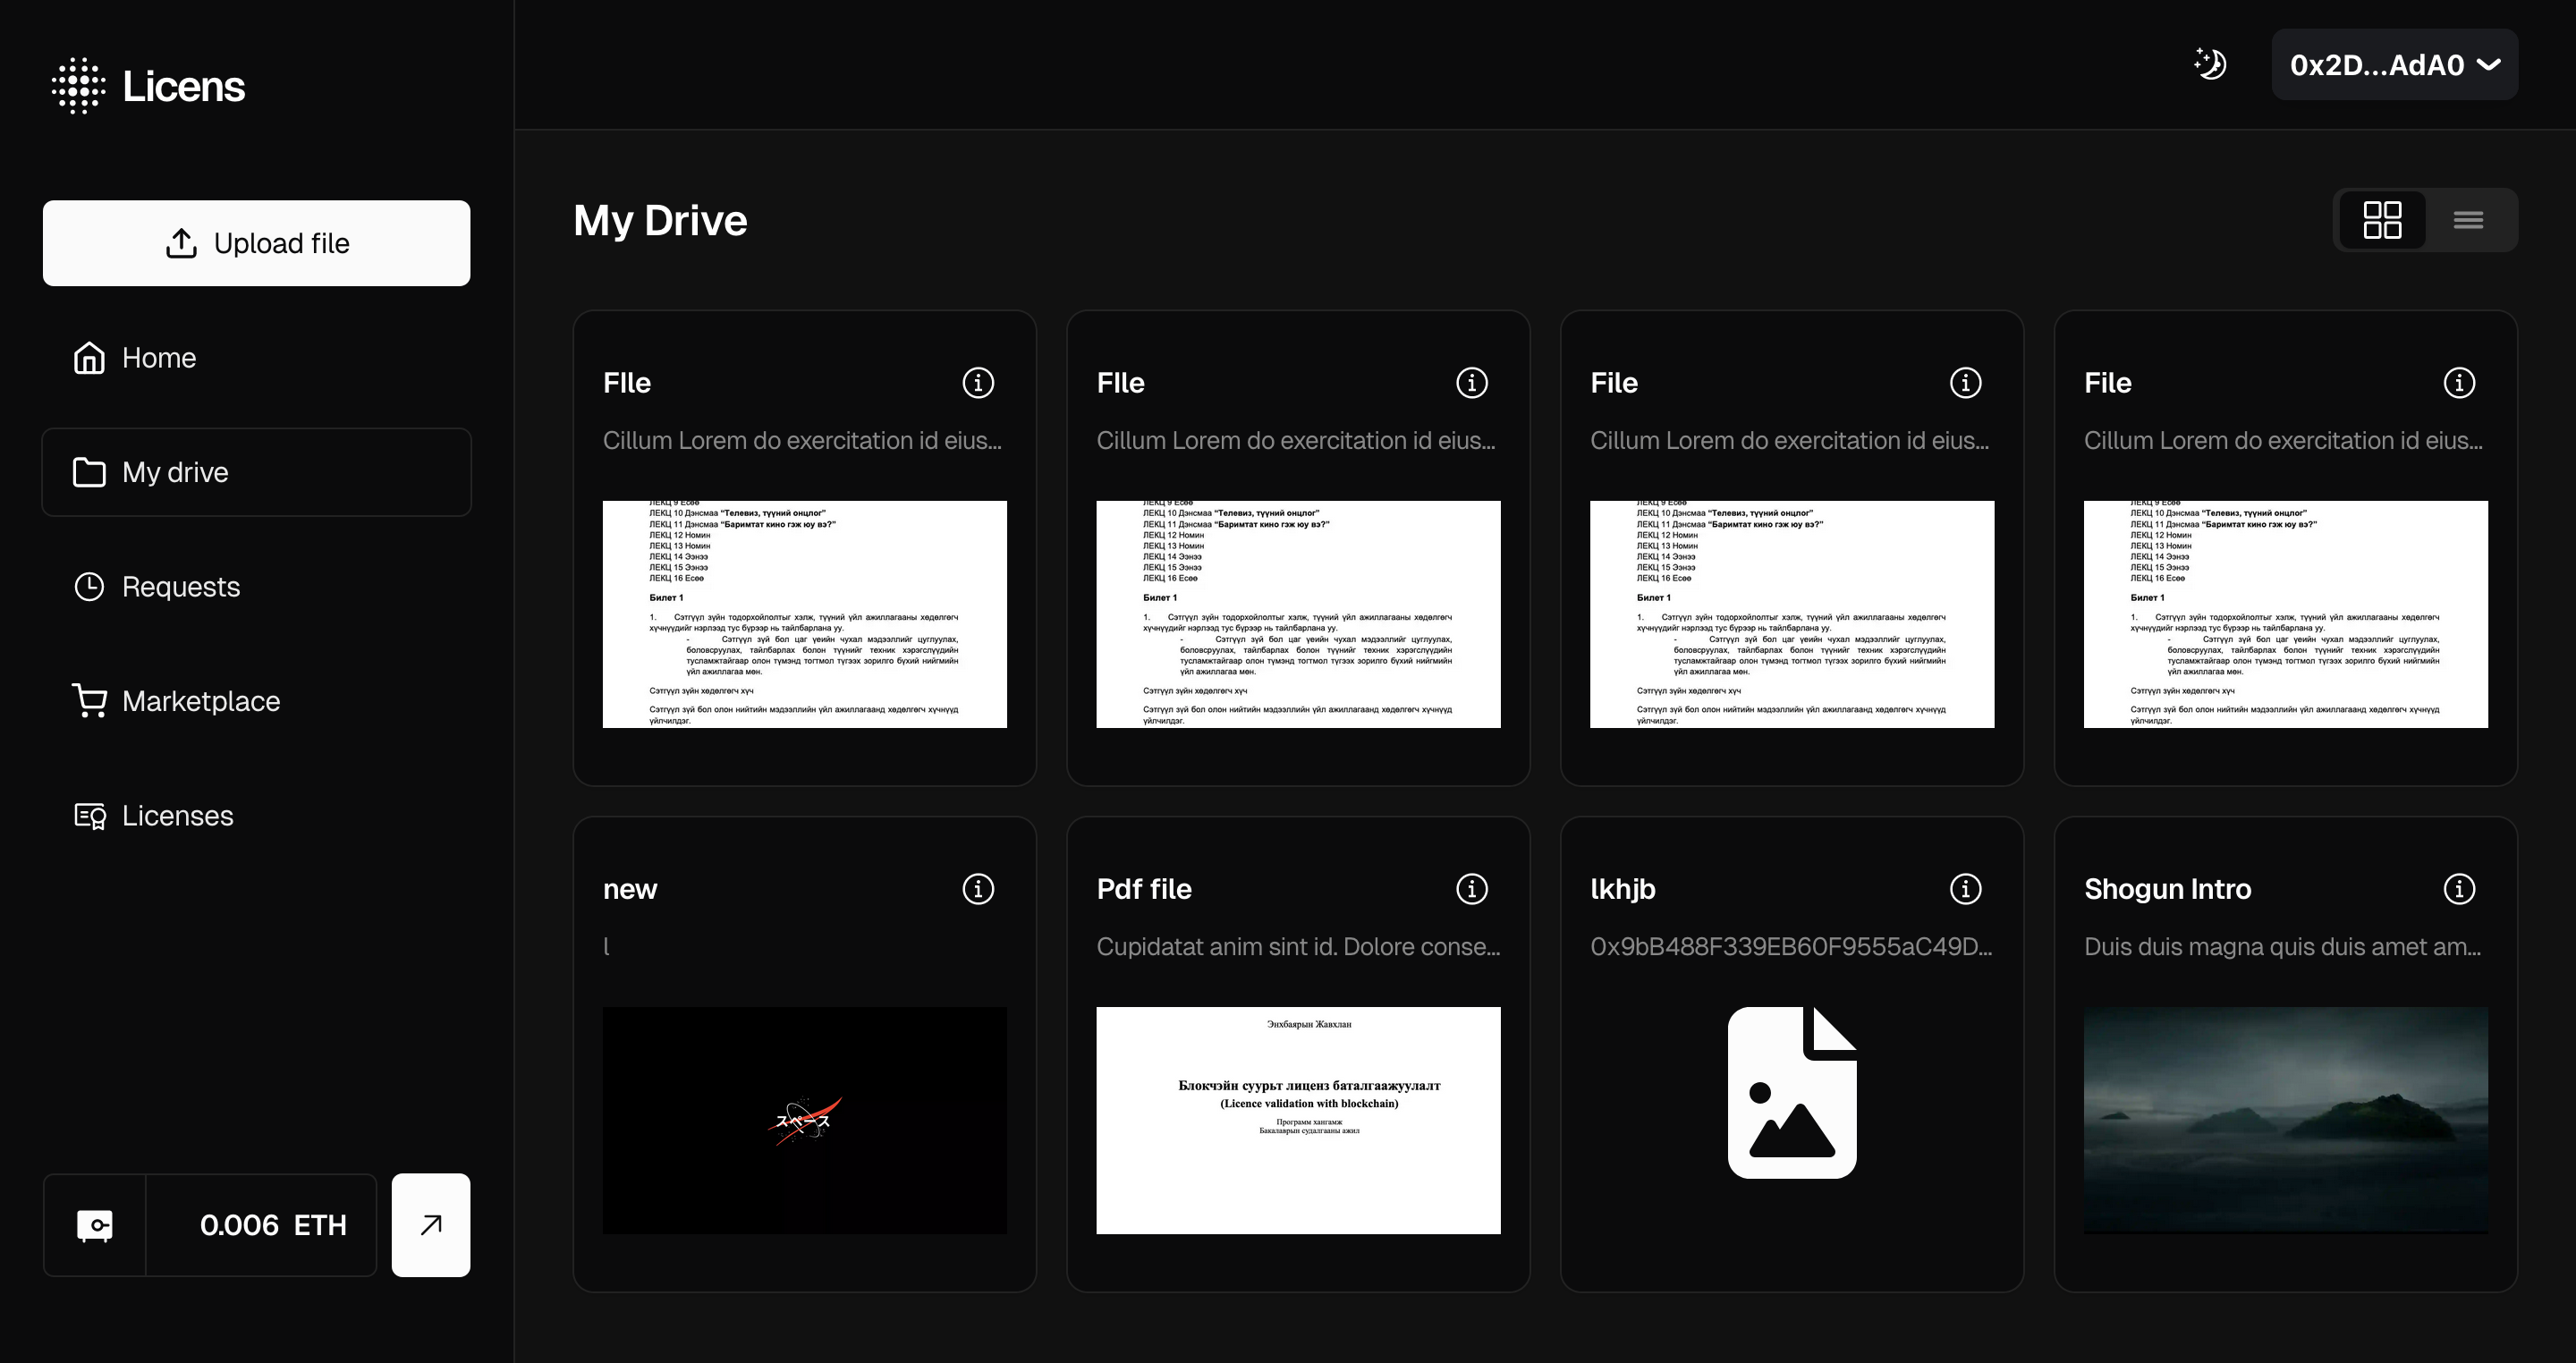
\includegraphics[scale=0.16]{src/images/drive.png}
	\caption{Миний сан хуудас}
\end{figure}

\begin{figure}[h!]
	\centering
	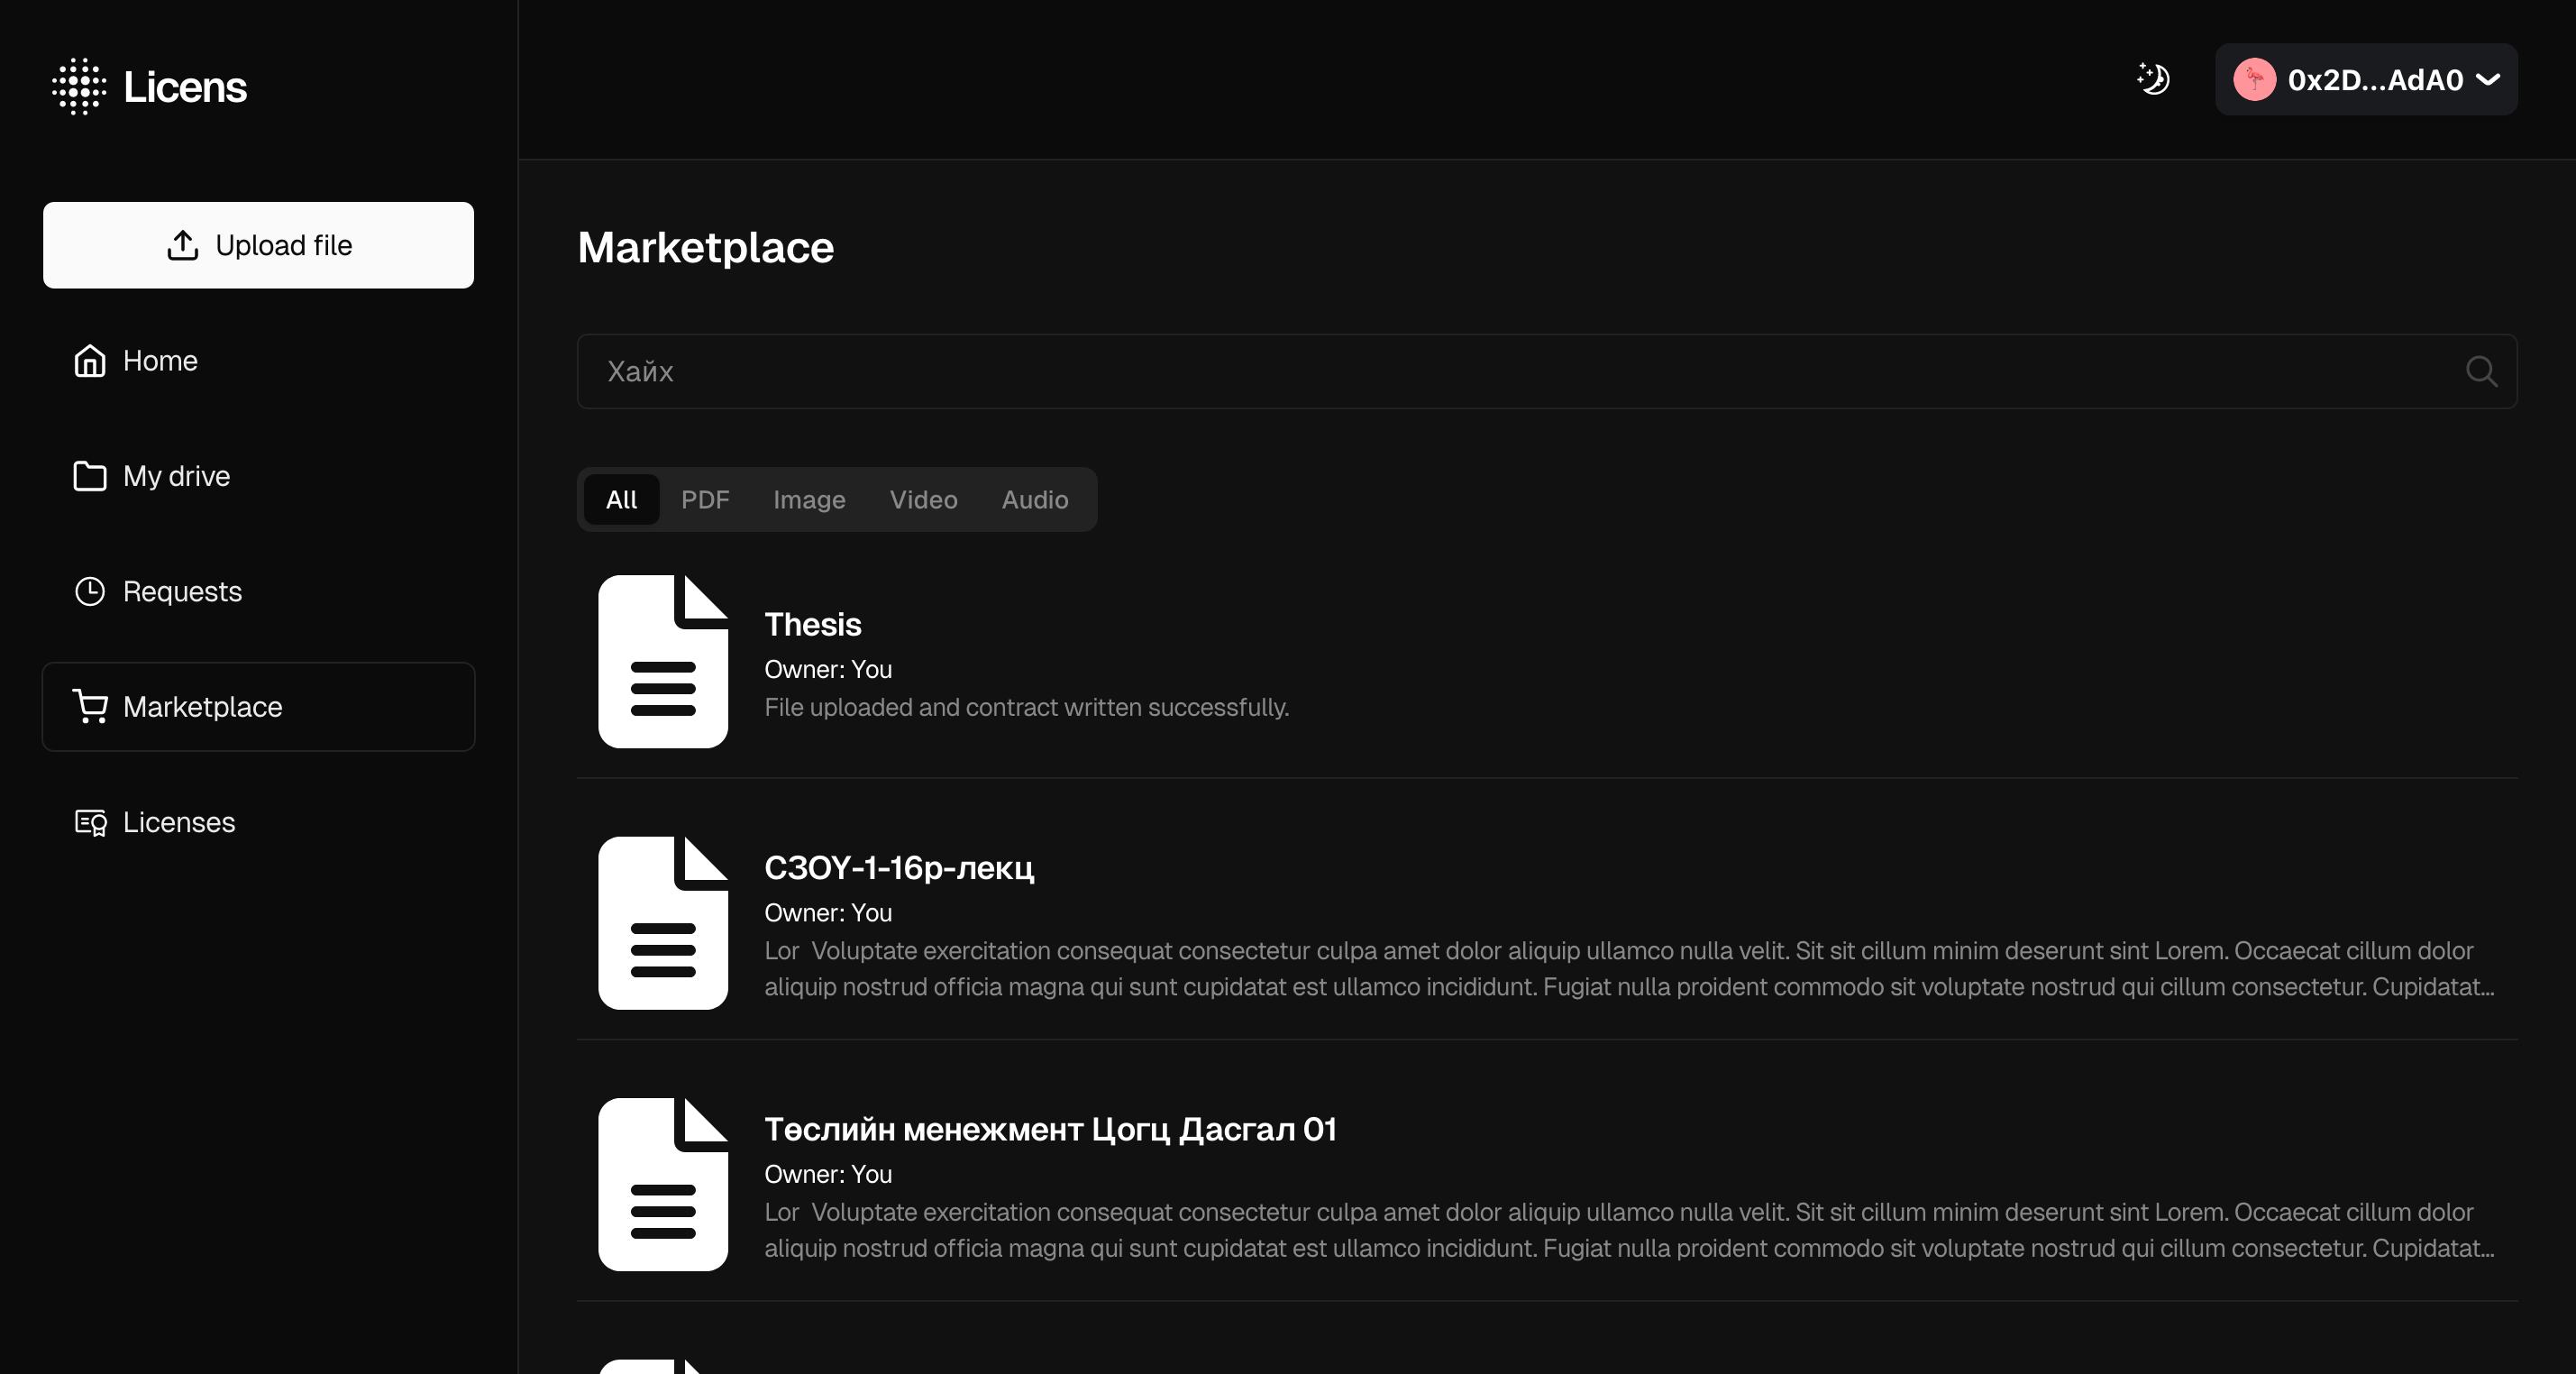
\includegraphics[scale=0.16]{src/images/marketplace.png}
	\caption{Marketplace хуудас}
\end{figure}

\begin{figure}[h!]
	\centering
	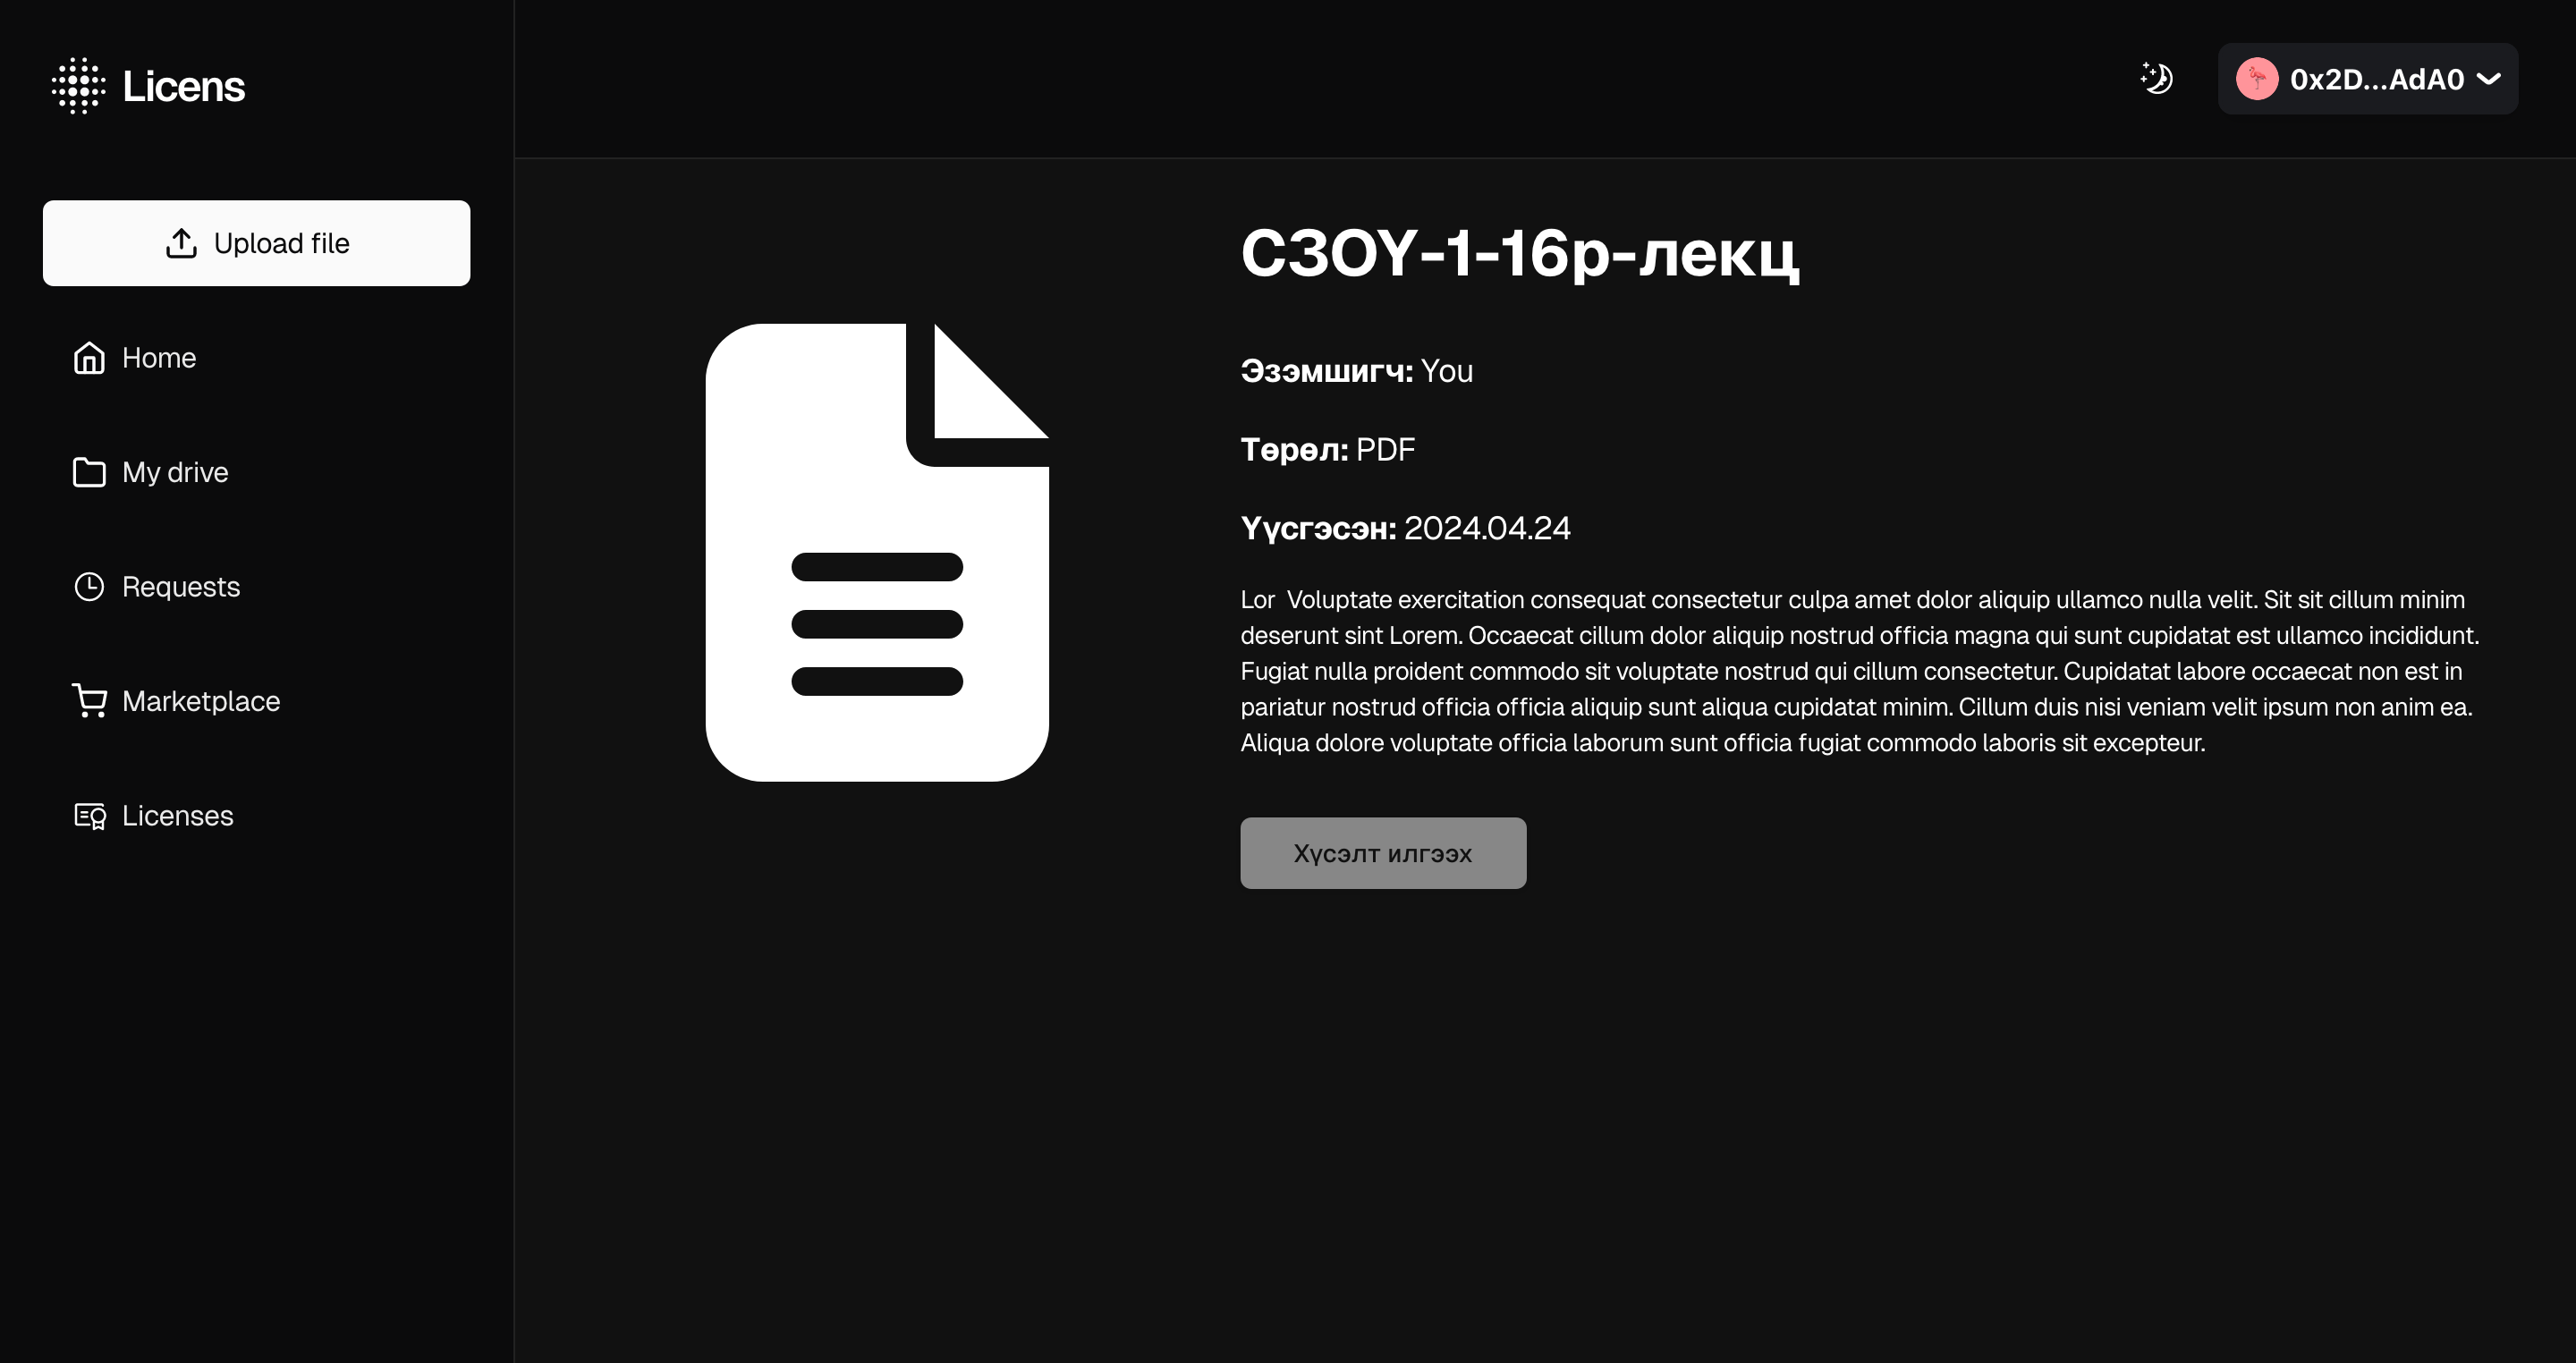
\includegraphics[scale=0.16]{src/images/marketplace-file.png}
	\caption{Marketplace дэх бүтээлийн хуудас}
\end{figure}

\begin{figure}[h!]
	\centering
	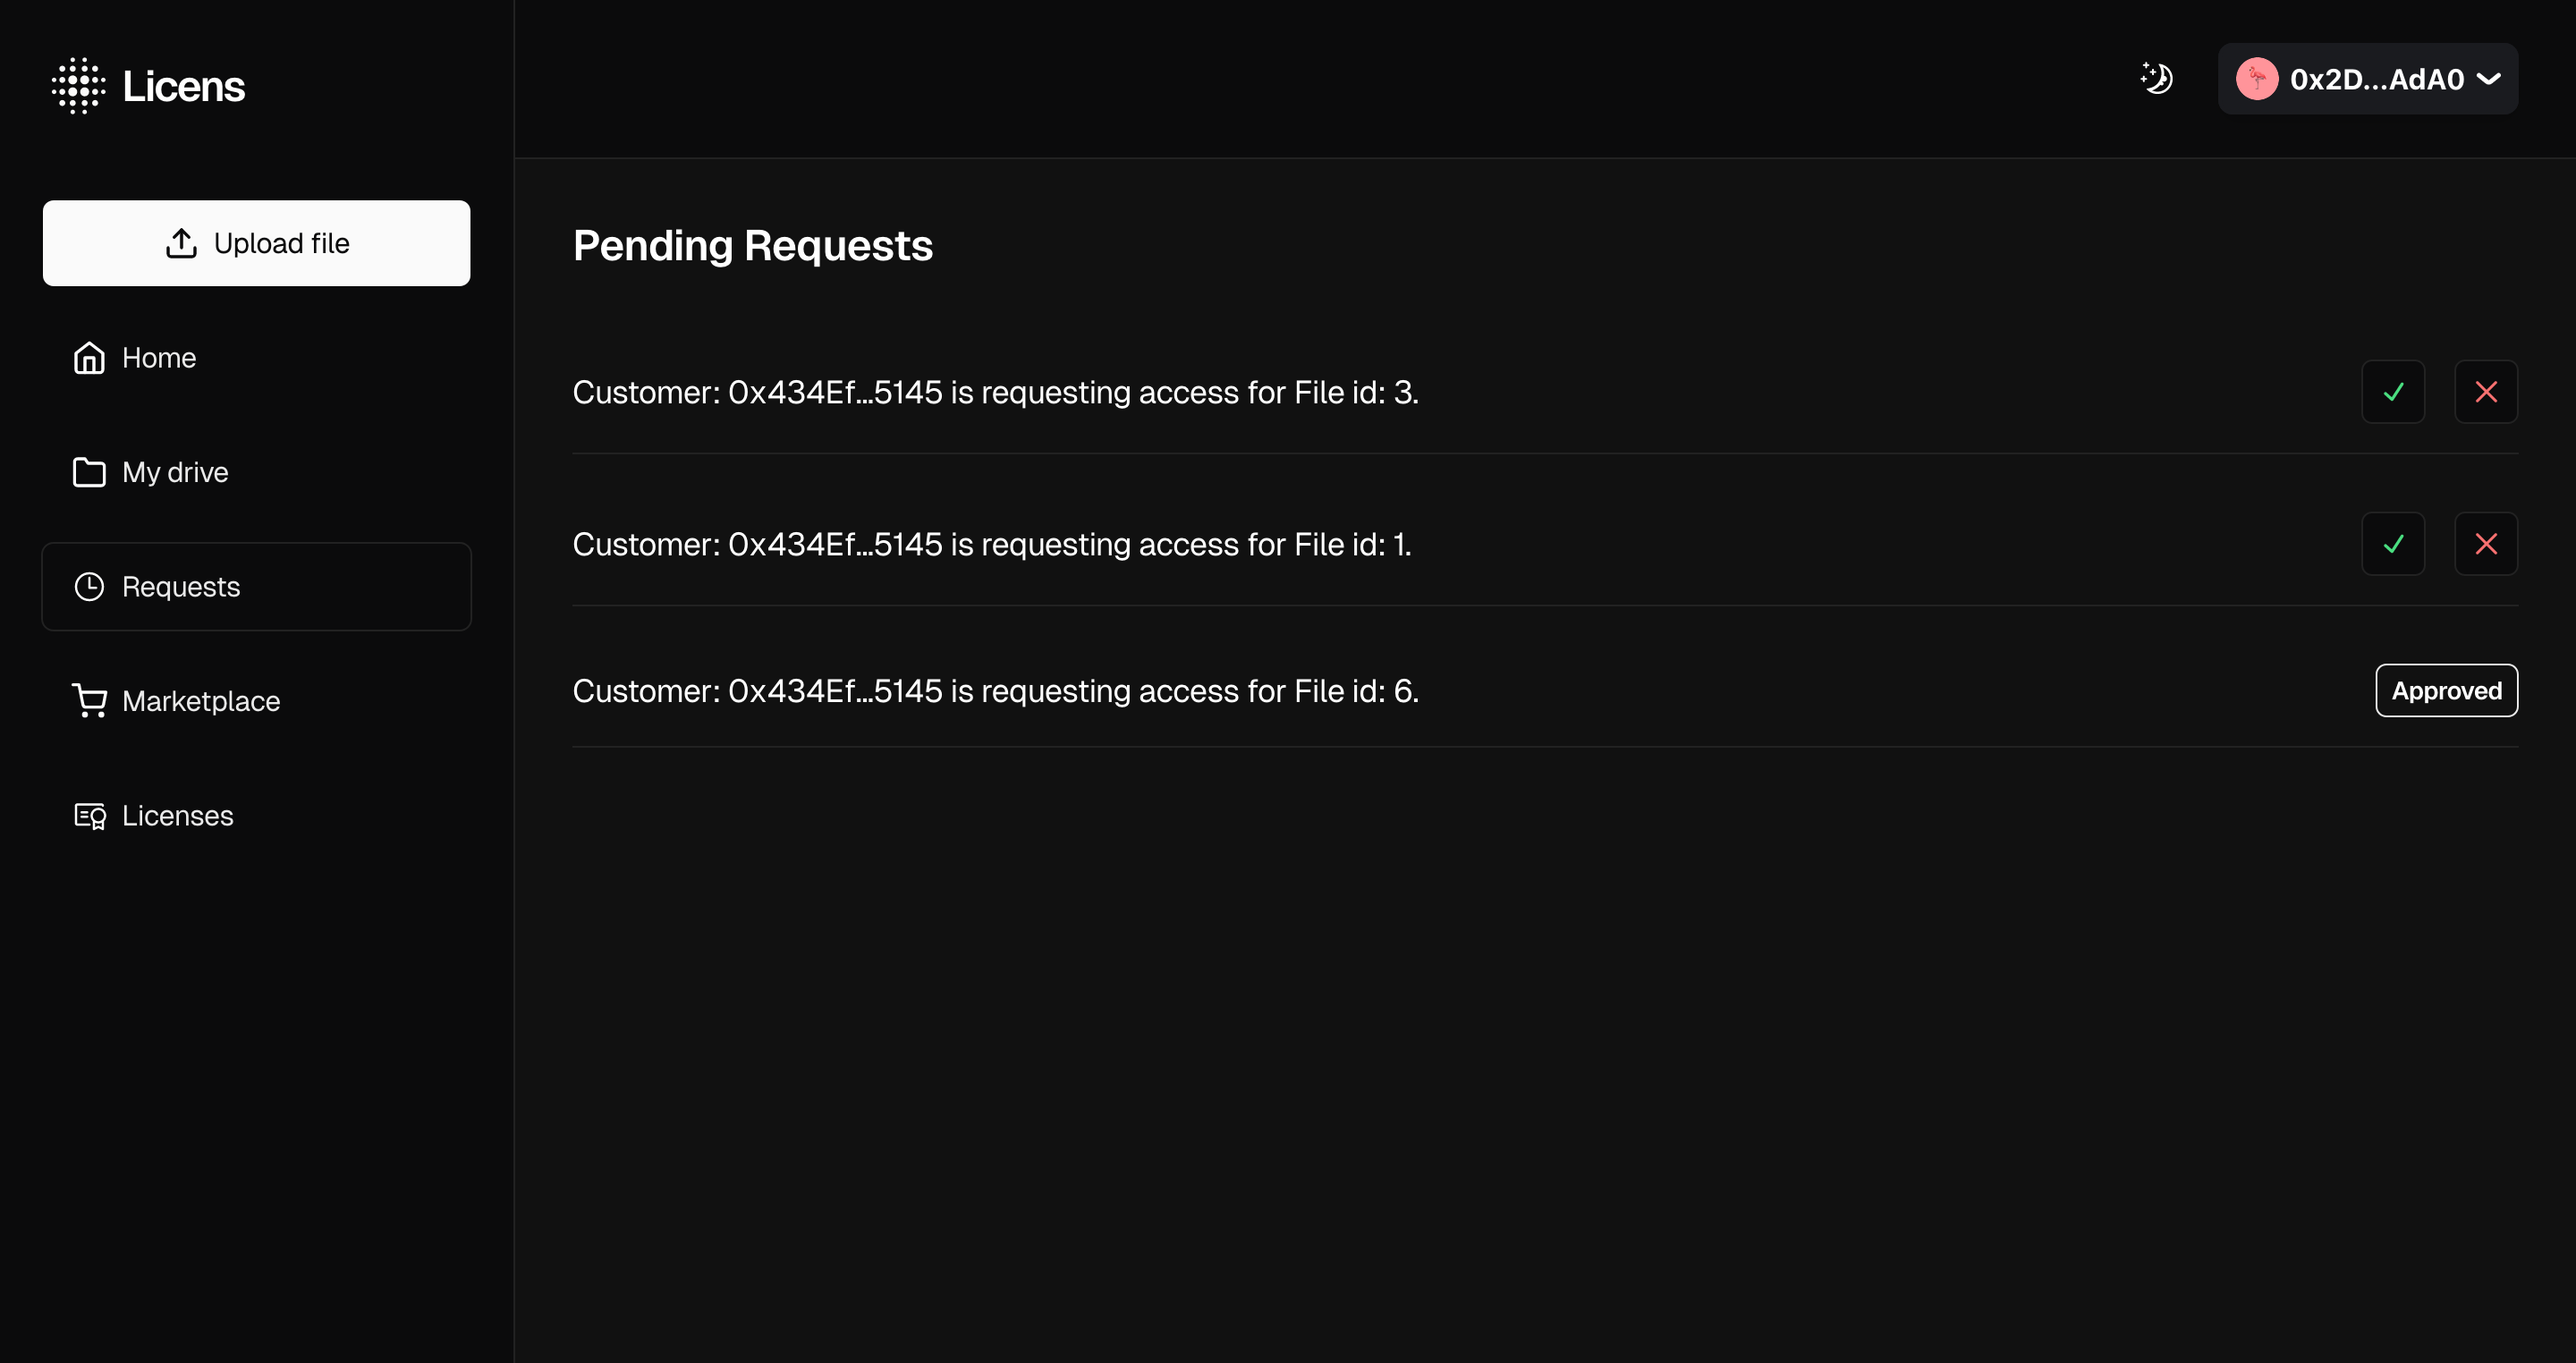
\includegraphics[scale=0.16]{src/images/requests.png}
	\caption{Лиценз хүсэлтийн  хуудас}
\end{figure}